\documentclass[11pt,a4paper]{article}

\usepackage[margin=2.3cm]{geometry}
\usepackage[T1]{fontenc}
\usepackage{lmodern}
\usepackage{microtype}
\usepackage{graphicx}
\usepackage{booktabs}
\usepackage{xcolor}
\usepackage{tikz}
\usetikzlibrary{arrows.meta,positioning,fit,calc}
\usepackage{caption}
\usepackage{enumitem}
\usepackage{amsmath}
\usepackage[hidelinks]{hyperref}
\usepackage{float}
\usepackage{tcolorbox}

\setlist{itemsep=2pt,topsep=4pt}
\captionsetup{font=small,labelfont=bf}
\definecolor{boxblue}{HTML}{E8F1FC}
\definecolor{boxline}{HTML}{2A78D6}
\definecolor{boxgreen}{HTML}{E7F6EF}
\definecolor{linegreen}{HTML}{1BAF7A}
\definecolor{boxorange}{HTML}{FDEEE7}
\definecolor{lineorange}{HTML}{EB6834}
\newtcolorbox{decision}[1]{colback=boxblue,colframe=boxline,boxrule=0.5pt,arc=2pt,left=4pt,right=4pt,top=2pt,bottom=2pt,
  fontupper=\small,title={\small\textbf{#1}},coltitle=black,colbacktitle=boxblue,titlerule=0pt,toptitle=1pt,bottomtitle=0pt}
\newtcolorbox{finding}{colback=boxgreen,colframe=linegreen,boxrule=0.5pt,arc=2pt,left=4pt,right=4pt,top=2pt,bottom=2pt,fontupper=\small}

\newcommand{\qSimExR}{40.0}
\newcommand{\qGemExR}{82.7}
\newcommand{\qSimImR}{58.5}
\newcommand{\qGemImR}{87.7}
\newcommand{\qSimExROne}{8.5}
\newcommand{\qGemExROne}{82.4}
\newcommand{\qGemLat}{15.6}
\newcommand{\qMxbaiExR}{77.9}
\newcommand{\qEFiveExR}{30.7}
\newcommand{\qReplyGap}{0.6}
\newcommand{\qMemEx}{98.6}
\newcommand{\qMemIm}{99.9}
\newcommand{\qFalseSixteen}{0.22}
\newcommand{\qFalseTwentyThree}{0.65}
\newcommand{\qMissedEx}{14}
\newcommand{\qLlExMemThree}{96.5}
\newcommand{\qLlExRagThree}{74.8}
\newcommand{\qLlImMemThree}{83.5}
\newcommand{\qLlImRagThree}{73.7}
\newcommand{\qLlExGemThree}{93.9}
\newcommand{\qMiMemTwentyThree}{88.6}
\newcommand{\qMiRagTwentyThree}{53.7}
\newcommand{\qMiRemTwentyThree}{46.9}
\newcommand{\qMiZsTwentyThree}{37.6}
\newcommand{\qMiMemTen}{93.7}
\newcommand{\qMiGainTwentyThree}{34.9}
\newcommand{\qMiImMemZero}{81.9}
\newcommand{\qMiImRemZero}{88.4}
\newcommand{\qMiImMemThree}{79.8}
\newcommand{\qMiImRagThree}{64.0}
\newcommand{\qLostEx}{49}
\newcommand{\qLostExParse}{40}
\newcommand{\qLostIm}{99}
\newcommand{\qLostImParse}{65}
\newcommand{\qLostImGold}{98}
\newcommand{\qMiCondTen}{94.5}
\newcommand{\qMiCondTwentyThree}{89.1}
\newcommand{\qMiMissAccLo}{36}
\newcommand{\qMiMissAccHi}{50}
\newcommand{\qStExAll}{90.5}
\newcommand{\qStExTop}{93.9}
\newcommand{\qStImAll}{71.1}
\newcommand{\qStImTop}{77.0}
\newcommand{\qStKeepEx}{97.4}
\newcommand{\qStKeepIm}{98.5}
\newcommand{\qTokZs}{3,282}
\newcommand{\qTokMem}{3,343}
\newcommand{\qTokAdd}{61}
\newcommand{\qClfLat}{1.4}
\newcommand{\qTotalQ}{46,000}
\newcommand{\qGpuHours}{44}

\graphicspath{{figures/}}

\title{\textbf{Improving Long-Context Preference Following in LLMs}\\[2pt]
\large Phase 3 Report: Preference Memory and Modern Retrieval}
\author{Krishna Jhanwar (12341250)\\ \small\texttt{krishnaj@iitbhilai.ac.in}}
\date{October 2026}

\begin{document}
\maketitle

\begin{abstract}
\noindent
Phase~3 combines the Phase~2 preference classifier and a modern embedding model into a \emph{preference memory}. It evaluates the result
against all five PrefEval baselines reproduced in Phase~1, on the same 1{,}000 questions per cell, with the same local models (Llama-3-8B,
Mistral-7B-v0.2), decoding and metric. The work has two steps.
\textbf{(1) Retrieval benchmark:} five current encoders are compared with the paper's SimCSE retriever, without any LLM calls. At 23k tokens,
EmbeddingGemma-2 finds the stated preference in its top~5 for \qGemExR\% of explicit questions, versus \qSimExR\% for SimCSE.
\textbf{(2) Memory pipeline:} the classifier (held out by topic) puts the true preference into memory for \qMemEx\% of explicit and
\qMemIm\% of implicit questions. Before each answer, the memory is written into the prompt as a short ``Known user preferences'' block.
Across \qTotalQ{} LLM-answered questions (about \qGpuHours{}~GPU-hours), memory beats every baseline at every length from 1k tokens up, for both models
and both preference forms, and is the best of all methods in 10 of these 11 cells. With Mistral at 23k tokens it reaches \qMiMemTwentyThree\% versus \qMiRagTwentyThree\% for the paper's RAG
(+\qMiGainTwentyThree{} points). With Llama at 3k it reaches \qLlExMemThree\% versus \qLlExRagThree\% (explicit) and \qLlImMemThree\% versus
\qLlImRagThree\% (implicit). Adding retrieved raw messages on top of memory does not help. A stress test with up to 20 unrelated preferences
in memory shows that retrieving the top~5 entries \emph{over the memory} keeps accuracy stable, whereas injecting every entry degrades it.
\end{abstract}

%===============================================================================
\section{Goal and where Phase 3 fits}
PrefEval~\cite{prefeval} shows that LLMs forget a user's stated preference as unrelated conversation piles up between the statement and a later
question. Phase~1 reproduced this locally: on the multiple-choice (MCQ) task, Llama-3-8B zero-shot falls from 94\% at 0.2k tokens to 43\% at 3k,
and even the paper's best method (RAG with a 2021 SimCSE retriever) falls to 54\% with Mistral at 23k. The proposal identified two weak points:
\textbf{long-context retrieval} (an old encoder) and \textbf{no persistent preference state} (every baseline re-reads the whole conversation at
question time). Phase~2 built a small classifier that flags preference-stating user turns. Phase~3 tests the proposal's full idea:

\begin{quote}\itshape
Flag preference turns with the classifier as they arrive, keep them in a memory list, and at question time put the memory (and retrieved context
from a better encoder) into the prompt. Then evaluate against the paper's baselines with the paper's own metric.
\end{quote}

Everything in Phase~3 is evaluated exactly like Phase~1: the PrefEval MCQ task, all 20 topics, 1{,}000 questions per form, the same Ollama models
(Q8, temperature~0, seed~41, raw prompts), the same option shuffle, and the same strict answer parser (\texttt{extract\_choice}).
The generation task stays out of scope, as in Phase~1, because its judge is Claude-3-Sonnet.

%===============================================================================
\section{The pipeline at a glance}
\begin{figure}[H]
\centering
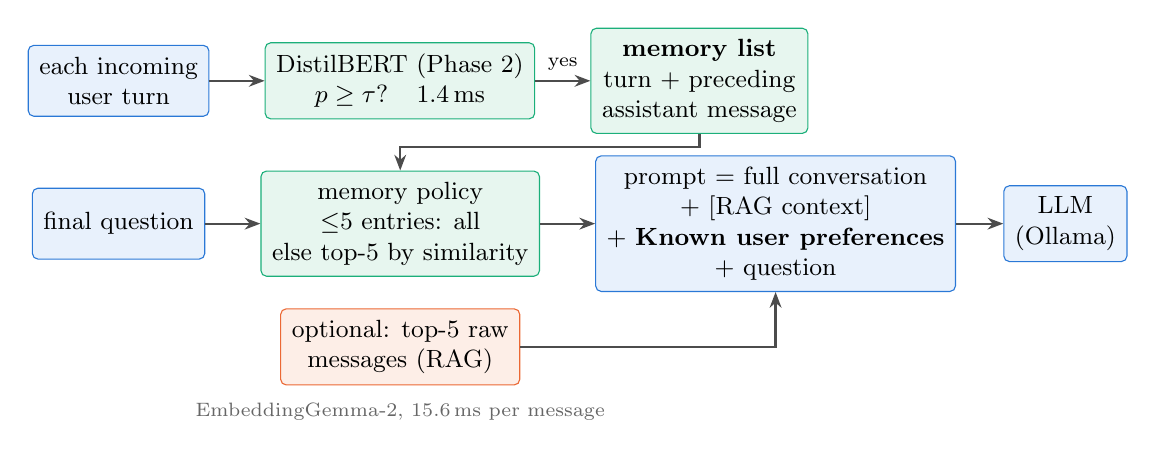
\begin{tikzpicture}[font=\small, node distance=4mm and 7mm,
  box/.style={draw=boxline, fill=boxblue, rounded corners=2pt, align=center, inner sep=4pt, minimum height=9mm},
  gbox/.style={draw=linegreen, fill=boxgreen, rounded corners=2pt, align=center, inner sep=4pt, minimum height=9mm},
  obox/.style={draw=lineorange, fill=boxorange, rounded corners=2pt, align=center, inner sep=4pt, minimum height=9mm},
  arr/.style={-{Stealth[length=2mm]}, thick, draw=black!70}]
\node[box] (turn) {each incoming\\user turn};
\node[gbox, right=of turn] (clf) {DistilBERT (Phase 2)\\$p \geq \tau$? \ \ \qClfLat\,ms};
\node[gbox, right=of clf] (mem) {\textbf{memory list}\\turn + preceding\\assistant message};
\node[box, below=9mm of turn] (q) {final question};
\node[gbox, right=of q] (sel) {memory policy\\$\leq$5 entries: all\\else top-5 by similarity};
\node[obox, below=of sel] (rag) {optional: top-5 raw\\messages (RAG)};
\node[box, right=of sel, minimum width=33mm] (prompt) {prompt = full conversation\\+ [RAG context]\\+ \textbf{Known user preferences}\\+ question};
\node[box, right=6mm of prompt] (llm) {LLM\\(Ollama)};
\draw[arr] (turn) -- (clf);
\draw[arr] (clf) -- node[above, font=\scriptsize]{yes} (mem);
\draw[arr] (mem.south) |- ($(sel.north)+(0,3mm)$) -- (sel.north);
\draw[arr] (q) -- (sel);
\draw[arr] (sel) -- (prompt);
\draw[arr] (rag.east) -| (prompt.south);
\draw[arr] (prompt) -- (llm);
\node[font=\scriptsize, text=black!60, below=1mm of rag] {EmbeddingGemma-2, \qGemLat\,ms per message};
\end{tikzpicture}
\caption{Phase 3 pipeline. Green: the new components (classifier, memory, policy). Orange: retrieval over raw messages, which is tested both with
and without memory. While the conversation runs, each user turn costs one classifier pass and one embedding; at question time, only a few entries are added to the prompt.}
\label{fig:pipeline}
\end{figure}

Phase~3 was built in two steps, and the second step's design depended on the first step's results:
\begin{enumerate}
  \item \textbf{Retrieval benchmark} (Section~\ref{sec:retrieval}, no LLM calls): which encoder finds the preference message best?
  \item \textbf{Memory and end-to-end runs} (Sections~\ref{sec:memory}--\ref{sec:results}): build memories with the classifier, write the prompts,
        and run the full Phase~1 grid plus a multi-preference stress test.
\end{enumerate}

%===============================================================================
\section{Step 1: retrieval benchmark}\label{sec:retrieval}

\subsection{Set-up}
\begin{itemize}
  \item \textbf{Question.} If we search a conversation with the final question, does the message that states the preference come back?
  \item \textbf{Candidates.} Every message before the question, one message per candidate, exactly as the paper's RAG does.
        Explicit: [preference, the LLM's own reply] + the first $2N$ LMSYS messages. Implicit-choice: [query, options, user's selection,
        acknowledgement] + $2N$ LMSYS messages. $N \in \{3, 8, 28, 48, 68\}$ are the paper's 1k--23k rows.
  \item \textbf{Gold.} The explicit preference sentence, or the user's selection turn for implicit-choice.
  \item \textbf{Metrics.} Recall@$k$ (is the gold message in the top $k$?), MRR, and latency to embed one message.
  \item \textbf{Retrievers.} The paper's SimCSE (RoBERTa-large), using the similarity scores stored in the upstream repository, and five current
        encoders: bge-base-v1.5, e5-base-v2, bge-large-v1.5, mxbai-embed-large-v1 and EmbeddingGemma-2.
\end{itemize}

\begin{decision}{Decisions and why}
\begin{itemize}[leftmargin=12pt]
  \item \textbf{One message = one retrieval unit}, as in the paper, so the comparison with SimCSE is like-for-like.
  \item \textbf{Each encoder's official query/document prompts}, taken from its model card or sentence-transformers config, and the
        \textbf{weights pinned to an exact commit}, so the run is reproducible.
  \item \textbf{Pre-computing embeddings is equivalent to real time.} A bi-encoder embeds every message independently, so a vector computed in
        advance equals the one computed when the message arrives. Only messages \emph{before} the question are candidates, so there is no look-ahead.
        The real-time cost is reported as per-message latency instead.
  \item \textbf{The LLM's own reply is in the pool.} The explicit pools contain the exact 5-token reply each LLM produced in Phase~1. The paper's
        stored SimCSE score for that position was computed on a \emph{different}, full reply. The two LLMs' pools give recall within
        \qReplyGap{} points of each other, so the pool for Llama is reported.
  \item \textbf{Same coverage as Phase~1 RAG.} SimCSE scores exist for 949 explicit and 973 implicit questions (one upstream file is truncated,
        and seven others end early). Every encoder is compared on exactly those questions.
\end{itemize}
\end{decision}

\paragraph{Verification.} Our SimCSE ranking reproduces the top~5 that upstream's own RAG code places in the prompt for all 9{,}610
(question, length) pairs. Re-encoding a sample matches the cached vectors to within $2\cdot10^{-7}$.

\subsection{Results}
\begin{table}[H]
\centering\small
\resizebox{\linewidth}{!}{\begin{tabular}{lr|ccccc|cccc|r}
\toprule
 & & \multicolumn{5}{c|}{Explicit} & \multicolumn{4}{c|}{Implicit-choice} &  \\
Retriever & Params & R@5 1k & 3k & 10k & 23k & R@1 23k & R@5 1k & 3k & 10k & 23k & ms/msg \\
\midrule
SimCSE (paper) & 355M & 0.95 & 0.83 & 0.60 & 0.40 & 0.05 & 0.97 & 0.90 & 0.75 & 0.58 & -- \\
\midrule
bge-base-v1.5 & 110M & 0.96 & 0.92 & 0.68 & 0.57 & 0.29 & 1.00 & 0.99 & 0.95 & 0.92 & 3.5 \\
e5-base-v2 & 110M & 0.96 & 0.86 & 0.44 & 0.31 & 0.12 & 1.00 & 1.00 & 0.96 & 0.93 & 3.6 \\
bge-large-v1.5 & 335M & 0.98 & 0.95 & 0.74 & 0.66 & 0.43 & 1.00 & 0.99 & 0.92 & 0.89 & 9.8 \\
mxbai-embed-large & 335M & 1.00 & 0.99 & 0.83 & 0.78 & 0.53 & 1.00 & 0.98 & 0.91 & 0.88 & 9.8 \\
\textbf{EmbeddingGemma-2} & 744M & 1.00 & 1.00 & 0.90 & 0.83 & 0.53 & 1.00 & 0.99 & 0.92 & 0.88 & 15.6 \\
\bottomrule
\end{tabular}
}
\caption{Retrieval of the preference message (recall@5 unless noted; questions with stored SimCSE scores). Latency = median ms to embed one
message (batch~1, RTX~3060, fp32).}
\label{tab:retrieval}
\end{table}

\begin{figure}[H]
\centering
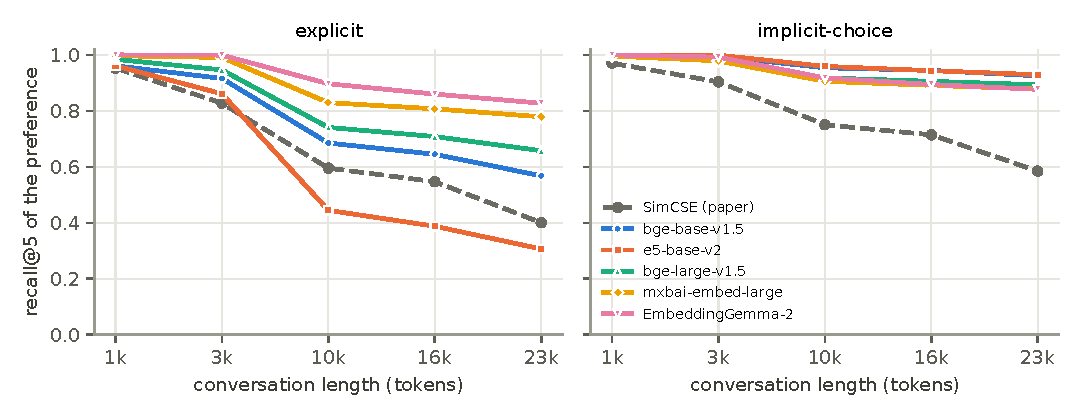
\includegraphics[width=0.92\linewidth]{p3_retrieval.pdf}
\caption{Recall@5 versus conversation length. Every modern encoder except e5-base degrades far more slowly than SimCSE.}
\label{fig:retrieval}
\end{figure}

\begin{finding}
\begin{itemize}[leftmargin=12pt]
  \item \textbf{The paper's retriever is the bottleneck at long context.} At 23k tokens, SimCSE finds the explicit preference in its top~5 for
        only \qSimExR\% of questions; EmbeddingGemma-2 finds it for \qGemExR\% (implicit: \qSimImR\% vs \qGemImR\%).
  \item \textbf{SimCSE almost never ranks the preference first.} Its recall@1 at 1k is \qSimExROne\% (EmbeddingGemma-2: \qGemExROne\%). It
        usually ranks the assistant's reply above the preference itself.
  \item \textbf{Newer is not automatically better.} e5-base-v2 falls \emph{below} SimCSE on long explicit conversations (\qEFiveExR\% at 23k).
  \item \textbf{On implicit, nobody ranks the user's selection first} (recall@1 of 5--28\%). The selection (``I'll go with the second one'') only
        makes sense together with the assistant's options message, which ranks higher. This shaped the memory design (Section~\ref{sec:memory}).
\end{itemize}
\end{finding}

\textbf{Choice: EmbeddingGemma-2} (best on explicit, close to the best on implicit, \qGemLat\,ms per message). mxbai-embed-large is a lighter
alternative at \qMxbaiExR\% (23k, explicit) and half the latency.

\paragraph{An upstream quirk found during verification.} The stored SimCSE \emph{scores} are consistent across files. However, in 13 of the 20 topics,
the explicit \texttt{msg\_index} file that maps a score index back to message text is shifted by one LMSYS exchange. In those topics, the paper's RAG
placed slightly different messages in the prompt than the ones it scored. Recall and rank depend only on the scores, so no number here changes;
Phase~1 reproduced upstream's behaviour as it is. Phase~3's own retrieval uses the real conversation order.

%===============================================================================
\section{Step 2: the preference memory}\label{sec:memory}
\begin{itemize}
  \item \textbf{Detection.} Every \emph{user} message before the question is scored by the Phase~2 DistilBERT classifier. A message enters memory
        when $p \geq \tau$, with $\tau$ tuned on validation topics in Phase~2.
  \item \textbf{No leakage.} Phase~2 trained five models with topic-level cross-validation. For a question from topic $t$ we use the model whose
        \emph{test} fold contains $t$, so the classifier has never seen that topic.
  \item \textbf{Entry = flagged turn + the assistant message just before it.} For implicit-choice, an entry is therefore the options list plus the
        user's selection, which is the context the retrieval benchmark showed the selection needs. An explicit preference is the first message,
        so it is stored alone.
  \item \textbf{Memory policy.} If the memory holds 5 entries or fewer, all of them go into the prompt. Otherwise, the 5 entries most similar
        to the question (EmbeddingGemma-2; an entry scores the highest similarity of its messages) go in, kept in conversation order.
\end{itemize}

\begin{table}[H]
\centering\small
\resizebox{\linewidth}{!}{\begin{tabular}{l|cccccc|ccc|c}
\toprule
 & \multicolumn{6}{c|}{True preference in memory (\%)} & \multicolumn{3}{c|}{False entries / question} & Mean size \\
Form & 0.2k & 1k & 3k & 10k & 16k & 23k & 10k & 16k & 23k & at 23k \\
\midrule
explicit & 98.6 & 98.6 & 98.6 & 98.6 & 98.6 & 98.6 & 0.00 & 0.22 & 0.65 & 1.63 \\
implicit-choice & 99.9 & 99.9 & 99.9 & 99.9 & 99.9 & 99.9 & 0.00 & 0.22 & 0.65 & 1.64 \\
\bottomrule
\end{tabular}
}
\caption{Memory quality (1{,}000 questions per cell). False entries come only from LMSYS messages, and only once the conversation reaches 16k tokens.}
\label{tab:memory}
\end{table}

The classifier catches the true preference in \qMemEx\% of explicit and \qMemIm\% of implicit questions (\qMissedEx{} explicit misses,
mostly preferences phrased as a dislike, such as ``I'm uncomfortable with invisible fences''). False entries appear only at 16k (\qFalseSixteen{} per
question) and 23k (\qFalseTwentyThree). They are two LMSYS messages that read like stated opinions (a product description, an opinion about art).
On PrefEval, memories therefore hold 1--3 entries, so the ``include all'' branch of the policy is what runs. Section~\ref{sec:stress} tests the other branch.

%===============================================================================
\section{Methods and prompts}\label{sec:methods}
\begin{decision}{Design rule: each new method changes exactly one thing compared with a Phase 1 baseline}
\begin{tabular}{@{}p{0.27\linewidth}p{0.68\linewidth}@{}}
\textbf{Memory} & upstream zero-shot prompt, with the ``Known user preferences'' block inserted before the question \\
\textbf{RAG, EmbeddingGemma-2} & upstream RAG prompt (same builder, same wording), with the top~5 from EmbeddingGemma-2 instead of SimCSE \\
\textbf{Memory + RAG} & the RAG prompt above, plus the memory block (retrieved context, then memory, then the question) \\
\end{tabular}
\end{decision}

The full conversation stays in every prompt, as in all baselines. The additions go into the final user turn, where upstream's RAG puts its
context. The memory block reads ``Known user preferences: these are the preferences I have stated before'', followed by numbered entries with their turn
numbers and ``Please follow these preferences wherever they are relevant to my question.'' It adds about \qTokAdd{} tokens to a \qTokZs-token
prompt (Llama, explicit, 3k).

\paragraph{Verification.} With SimCSE's picks substituted, our RAG prompt is \emph{byte-identical} to Phase~1's RAG prompt. With an empty memory,
our memory prompt is byte-identical to Phase~1's zero-shot prompt. Both hold for 96 checked prompts across both models and both forms. Every
accuracy difference is therefore caused by the change itself, not by the prompt plumbing.

\paragraph{Other implementation decisions.}
\begin{itemize}
  \item \textbf{The LLM's reply to the stated preference is reused from Phase~1} (explicit form). Decoding is deterministic and the reply was
        identical in every Phase~1 method and length; regenerating it in a smoke test matched exactly. This saves one LLM call per question.
  \item \textbf{The strict metric is kept}, even though it penalises answers that are correct but badly formatted (Section~\ref{sec:whyrag}).
        Changing it would break comparability with Phase~1 and the paper. A lenient parse is logged as a diagnostic.
  \item \textbf{Same Ollama settings as each model's baselines} (Llama: defaults; Mistral: flash attention + q8\_0 KV cache, 32k context),
        enforced by Phase~1's settings guard.
  \item \textbf{RAG at 0.2k is skipped}, as in Phase~1, because there are too few messages to retrieve from.
\end{itemize}

%===============================================================================
\section{Experimental grid}
The grid mirrors Phase~1 exactly, so every Phase~3 cell has baselines on the same questions. Runs were split into tiers that each fit in one
overnight session and resume per question (Table~\ref{tab:tiers}).

\begin{table}[H]
\centering\small
\resizebox{\linewidth}{!}{\begin{tabular}{llllrr}
\toprule
Tier & Model & Forms & Lengths and methods & Questions & Hours \\
\midrule
A & Llama-3-8B & explicit, implicit & 0.2k--3k; memory, RAG-Gemma, memory+RAG & 14{,}000 & 5.6 \\
S & Llama-3-8B & explicit, implicit & 3k; stress test, $D\in\{5,10,20\}$ $\times$ 2 policies & 12{,}000 & 7.9 \\
B2 & Mistral-7B & explicit & 10k--23k; memory & 3{,}000 & 11.8 \\
B & Mistral-7B & explicit & 10k--23k; memory+RAG & 3{,}000 & 12.2 \\
C\_short & Mistral-7B & explicit, implicit & 0.2k--3k; all three methods & 14{,}000 & 6.3 \\
\midrule
 & & & & \qTotalQ & \qGpuHours \\
\bottomrule
\end{tabular}}
\caption{Runs. Not run: RAG-Gemma alone for Mistral at 10k--23k (optional tier C\_long, about 12\,h).}
\label{tab:tiers}
\end{table}

%===============================================================================
\section{Results}\label{sec:results}

\subsection{Main comparison with the Phase 1 baselines}
\begin{table}[H]
\centering\small
\begin{tabular}{l|ccc|ccc}
\toprule
 & \multicolumn{3}{c|}{Explicit} & \multicolumn{3}{c}{Implicit-choice} \\
Method & 0.2k & 1k & 3k & 0.2k & 1k & 3k \\
\midrule
Zero-shot & 94.2 & 52.7 & 43.3 & 77.0 & 53.3 & 46.0 \\
Reminder & 97.4 & 78.0 & 59.4 & \textbf{91.0} & 77.0 & 60.3 \\
CoT & 93.7 & 78.0 & 63.9 & 84.4 & 70.3 & 61.7 \\
Self-Critic & 78.8 & 50.1 & 46.7 & 66.1 & 50.1 & 38.7 \\
RAG, SimCSE (paper) & -- & 88.6 & 74.8 & -- & 82.8 & 73.7 \\
\midrule
\textbf{Memory (ours)} & \textbf{97.7} & \textbf{96.0} & \textbf{96.5} & 90.0 & \textbf{86.3} & \textbf{83.5} \\
RAG, EmbeddingGemma-2 (ours) & -- & 94.7 & 93.9 & -- & 83.6 & 79.1 \\
Memory + RAG (ours) & -- & 93.4 & 92.9 & -- & 84.2 & 75.4 \\
\bottomrule
\end{tabular}

\caption{Llama-3-8B, accuracy \% (macro over 20 topics). Bold = best in the column. Phase~1 RAG covers the 949/973 questions with SimCSE scores;
all other cells cover 1{,}000.}
\label{tab:llama}
\end{table}

\begin{table}[H]
\centering\small
\begin{tabular}{l|cccccc}
\toprule
 & \multicolumn{6}{c}{Explicit} \\
Method & 0.2k & 1k & 3k & 10k & 16k & 23k \\
\midrule
Zero-shot & 95.5 & 61.5 & 55.5 & 42.5 & 37.1 & 37.6 \\
Reminder & 96.2 & 78.9 & 71.3 & 56.7 & 43.9 & 46.9 \\
CoT & 88.0 & 74.9 & 67.0 & -- & -- & -- \\
Self-Critic & 79.8 & 67.0 & 61.0 & -- & -- & -- \\
RAG, SimCSE (paper) & -- & 81.0 & 75.7 & 64.6 & 59.0 & 53.7 \\
\midrule
\textbf{Memory (ours)} & \textbf{97.1} & \textbf{94.7} & \textbf{94.9} & 93.7 & \textbf{92.4} & \textbf{88.6} \\
RAG, EmbeddingGemma-2 (ours) & -- & 85.3 & 86.1 & -- & -- & -- \\
Memory + RAG (ours) & -- & 94.2 & 94.4 & \textbf{94.1} & 90.6 & 87.5 \\
\bottomrule
\end{tabular}
\\[6pt]
\begin{tabular}{l|ccc}
\toprule
 & \multicolumn{3}{c}{Implicit-choice} \\
Method & 0.2k & 1k & 3k \\
\midrule
Zero-shot & 81.0 & 50.8 & 47.5 \\
Reminder & \textbf{88.4} & 71.9 & 63.1 \\
CoT & 74.0 & 60.2 & 59.5 \\
Self-Critic & 67.2 & 51.8 & 50.9 \\
RAG, SimCSE (paper) & -- & 69.0 & 64.0 \\
\midrule
\textbf{Memory (ours)} & 81.9 & \textbf{81.4} & \textbf{79.8} \\
RAG, EmbeddingGemma-2 (ours) & -- & 67.2 & 65.0 \\
Memory + RAG (ours) & -- & 79.3 & 78.3 \\
\bottomrule
\end{tabular}

\caption{Mistral-7B-v0.2, accuracy \%. CoT and Self-Critic were not run at 10k--23k in Phase~1, as in the paper.}
\label{tab:mistral}
\end{table}

\begin{figure}[H]
\centering
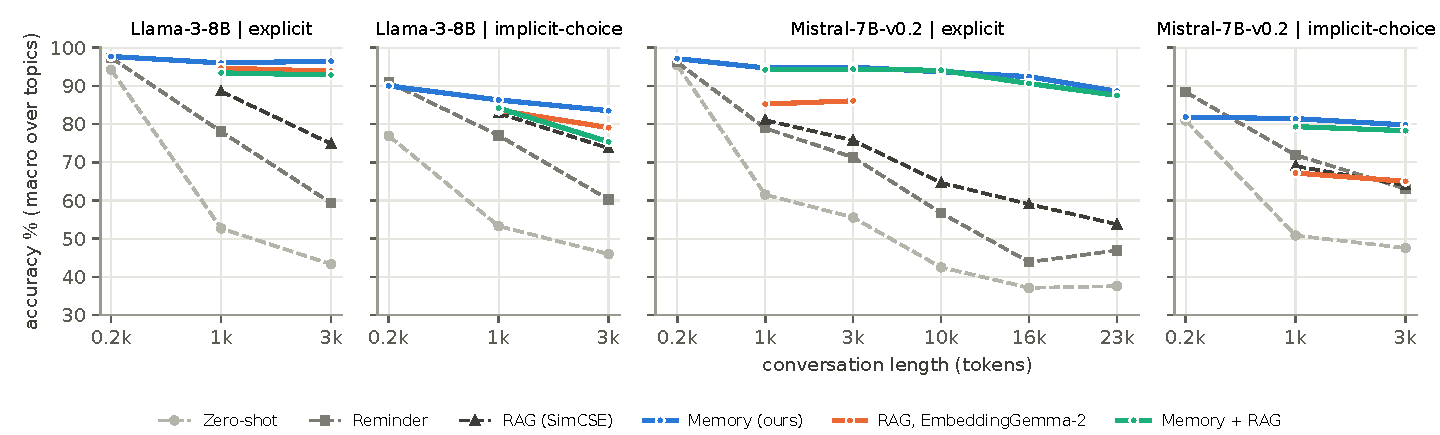
\includegraphics[width=\linewidth]{p3_main.pdf}
\caption{Accuracy versus conversation length. Dashed gray: Phase~1 baselines; solid: Phase~3 methods. Memory (blue) stays nearly flat while every
baseline declines.}
\label{fig:main}
\end{figure}

\begin{finding}
\begin{itemize}[leftmargin=12pt]
  \item \textbf{Memory beats every Phase~1 baseline at every length from 1k tokens up}, for both models and both forms (11 of 11 cells). It is
        the best of all methods in 10 of them; at Mistral 10k, memory + RAG is 0.4 points higher.
  \item \textbf{It removes most of the long-context collapse.} With Mistral at 23k tokens, memory reaches \qMiMemTwentyThree\% versus
        \qMiRagTwentyThree\% for the paper's RAG, \qMiRemTwentyThree\% for Reminder and \qMiZsTwentyThree\% for zero-shot. Between 0.2k and 23k,
        zero-shot and Reminder lose 49--58 points; memory loses 8.5.
  \item \textbf{At 0.2k there is nothing to forget.} With no distractor turns, memory ties with the best baseline on explicit, and on implicit it
        is not better: Mistral Reminder \qMiImRemZero\% vs memory \qMiImMemZero\%, Llama 91.0 vs 90.0. Its value is specifically in long conversations.
\end{itemize}
\end{finding}

\subsection{The better retriever on its own}
Holding the prompt fixed and swapping only the retriever, on identical questions:
\begin{table}[H]
\centering\small
\resizebox{\linewidth}{!}{\begin{tabular}{lll|cc|c|c}
\toprule
Model & Form & Length & SimCSE RAG & EmbeddingGemma-2 RAG & $\Delta$ & Memory + RAG \\
\midrule
Llama-3-8B & explicit & 1k & 88.6 & 94.6 & +6.0 & 93.2 \\
Llama-3-8B & explicit & 3k & 74.8 & 93.9 & +19.1 & 92.7 \\
Llama-3-8B & implicit-choice & 1k & 82.8 & 84.1 & +1.2 & 84.5 \\
Llama-3-8B & implicit-choice & 3k & 73.7 & 79.6 & +6.0 & 75.8 \\
Mistral-7B-v0.2 & explicit & 1k & 81.0 & 85.5 & +4.5 & 94.2 \\
Mistral-7B-v0.2 & explicit & 3k & 75.7 & 86.3 & +10.6 & 94.5 \\
Mistral-7B-v0.2 & implicit-choice & 1k & 69.0 & 67.6 & -1.4 & 79.3 \\
Mistral-7B-v0.2 & implicit-choice & 3k & 64.0 & 65.6 & +1.6 & 78.2 \\
\bottomrule
\end{tabular}
}
\caption{RAG with SimCSE (Phase~1) vs RAG with EmbeddingGemma-2 (Phase~3), same prompt builder, same questions.}
\label{tab:ragsame}
\end{table}
The new encoder helps a lot on \textbf{explicit} (Llama at 3k: \qLlExRagThree{}~$\rightarrow$~\qLlExGemThree), in line with Step~1. On \textbf{implicit} the gain is
small for Llama and absent for Mistral, even though retrieval itself improved (Table~\ref{tab:retrieval}). For implicit preferences the RAG prompt
format, not the retriever, is the limit: retrieved fragments of a choice dialogue are harder to use than an explicit statement. Memory reaches
\qMiImMemThree\% with Mistral at 3k, versus \qMiImRagThree\% for the paper's RAG.

\subsection{Why adding RAG on top of memory does not help}\label{sec:whyrag}
Memory + RAG is never clearly better than memory alone, and with Llama it is several points worse. To find out why, we compared the two methods
question by question (Table~\ref{tab:lost}).
\begin{table}[H]
\centering\small
\resizebox{\linewidth}{!}{\begin{tabular}{lll|cccc|c|c}
\toprule
Model & Form & Length & Lost & of which format & wrong option & pref.\ retrieved & Gained & Same answer \% \\
\midrule
Llama-3-8B & explicit & 3k & 49 & 40 & 9 & 49 & 11 & 93.8 \\
Llama-3-8B & implicit-choice & 3k & 99 & 65 & 34 & 98 & 16 & 85.2 \\
Mistral-7B-v0.2 & explicit & 3k & 14 & 0 & 14 & 14 & 7 & 97.5 \\
Mistral-7B-v0.2 & explicit & 23k & 28 & 0 & 28 & 22 & 16 & 95.1 \\
Mistral-7B-v0.2 & implicit-choice & 3k & 46 & 1 & 45 & 46 & 26 & 90.0 \\
\bottomrule
\end{tabular}
}
\caption{Questions answered correctly by memory but not by memory + RAG (``Lost''), split into format failures (no parseable
\texttt{<choice>}) and a wrong option. ``Pref.\ retrieved'' = the preference was in the retrieved top~5. ``Gained'' = the reverse case.}
\label{tab:lost}
\end{table}
\begin{itemize}
  \item \textbf{With Llama, most losses are format failures, not wrong preferences} (\qLostImParse{} of \qLostIm{} implicit, \qLostExParse{}
        of \qLostEx{} explicit at 3k). With two long context blocks, Llama starts writing ``Based on your previous\ldots'' instead of
        \texttt{<choice>X</choice>}, and the paper's 5-token answer budget cuts it off. This is the same failure mode behind the paper's RAG parse failures in Phase~1.
  \item \textbf{Retrieval did not fail.} The preference was in the retrieved context for \qLostImGold{} of the \qLostIm{} lost implicit questions.
  \item \textbf{Mistral has no format failures,} because its template pre-fills \texttt{<choice>}. There, the two methods give the same answer on
        90--98\% of questions, and the retrieved LMSYS messages occasionally pull it toward another option.
\end{itemize}
\textbf{Conclusion:} once the classifier has put the preference into memory, retrieving raw messages adds noise rather than information. The proposal
argued retrieval would act as a fallback for classifier misses. With about 99\% classifier recall there is little to fall back for, and the cost is
a longer, more distracting prompt.

\subsection{Where the remaining errors come from (Mistral, long context)}
For the questions whose preference reached memory, Mistral's accuracy still drops from \qMiCondTen\% at 10k to \qMiCondTwentyThree\% at 23k. So
the long conversation itself still distracts the model somewhat, even with the preference restated next to the question; the extra false memory
entries at 23k may contribute. The 14 questions the classifier missed are answered correctly only \qMiMissAccLo--\qMiMissAccHi\% of the time at
10k--23k, which is close to the no-help baselines. The classifier's errors cost little overall, simply because there are so few of them.

\subsection{Multi-preference stress test}\label{sec:stress}
On PrefEval every conversation contains one preference, so memories stay tiny. Real users state many preferences. To test the memory policy we
added $D$ preferences from questions of \emph{other} topics, as if stated in earlier sessions. Same-topic preferences were excluded because they can
contradict the true one and make the answer ambiguous. The sets are nested (the 5 are part of the 10, which are part of the 20), and entries appear
in a seeded random order with no turn labels, so position gives no hint. Llama-3-8B, 3k tokens, memory-only prompt.

\begin{table}[H]
\centering\small
\begin{tabular}{lc|cc|cc}
\toprule
 & & \multicolumn{2}{c|}{Include all} & \multicolumn{2}{c}{Top-5 retrieval over memory} \\
Form & $D$ & entries & accuracy & pref.\ kept (\%) & accuracy \\
\midrule
explicit & 0 & 1 & 96.5 & 100.0 & 96.5 \\
 & 5 & 6 & \textbf{94.3} & 100.0 & 94.2 \\
 & 10 & 11 & 92.8 & 99.1 & \textbf{93.8} \\
 & 20 & 21 & 90.5 & 97.4 & \textbf{93.9} \\
\midrule
implicit-choice & 0 & 1 & 83.5 & 100.0 & 83.5 \\
 & 5 & 6 & 77.1 & 100.0 & \textbf{78.0} \\
 & 10 & 11 & 73.7 & 99.9 & \textbf{77.7} \\
 & 20 & 21 & 71.1 & 98.5 & \textbf{77.0} \\
\bottomrule
\end{tabular}

\caption{Accuracy with $D$ extra preferences. ``Pref.\ kept'' = share of questions (whose preference reached memory) where top-5 retrieval over
the memory still selects it (no LLM calls, all 1{,}000 questions). Bold = better policy.}
\label{tab:stress}
\end{table}

\begin{figure}[H]
\centering
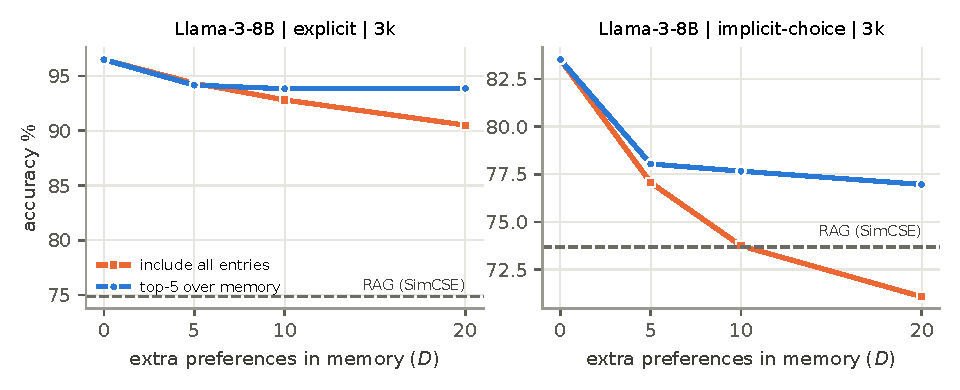
\includegraphics[width=0.78\linewidth]{p3_stress.pdf}
\caption{Injecting every memory entry degrades steadily; retrieving the top~5 over the memory levels off after $D = 5$.}
\label{fig:stress}
\end{figure}

\begin{finding}
\begin{itemize}[leftmargin=12pt]
  \item \textbf{Retrieval over the memory makes it scale.} With 20 extra preferences, ``include all'' drops to \qStExAll\% (explicit) and
        \qStImAll\% (implicit). Top-5 retrieval holds \qStExTop\% and \qStImTop\%, keeping the true preference for \qStKeepEx\% and \qStKeepIm\%
        of questions. This confirms the proposal's idea that a large memory should be searched, not dumped into the prompt.
  \item \textbf{The drop under ``include all'' is dilution, not missing information.} The true preference is in the prompt for every question
        whose preference reached memory, yet similar-looking preferences confuse the model. Implicit entries (an options list plus a selection)
        are long, so they suffer more.
  \item Even the hardest setting stays above the paper's RAG at the same length (explicit \qStExTop{} vs \qLlExRagThree; implicit \qStImTop{} vs
        \qLlImRagThree).
\end{itemize}
\end{finding}

\subsection{Cost}
Each incoming user turn costs one DistilBERT pass (\qClfLat\,ms) and one EmbeddingGemma-2 embedding (\qGemLat\,ms) on the GPU. Phase~2 measured
a prompted Llama-3-8B detector at about 51$\times$ the classifier's per-message time (72\,ms vs \qClfLat\,ms). At question time, memory adds about
\qTokAdd{} prompt tokens, and the measured time per question is no higher than zero-shot (Llama, 3k: 1.9\,s vs 2.0\,s). Unlike the paper's RAG, memory adds no retrieval step when the memory is small.

%===============================================================================
\section{Answers to the proposal's questions}
\begin{itemize}
  \item \textbf{Does a trained classifier + memory beat the paper's baselines?} Yes, at every length from 1k up, for both models and forms; by up to
        35 points at 23k.
  \item \textbf{Does a modern encoder improve RAG?} Yes for explicit preferences (up to +19 points), but barely for implicit ones, where the RAG prompt
        format limits accuracy.
  \item \textbf{Is retrieval still needed alongside memory?} Not over raw messages on this benchmark: the classifier's recall is high enough that
        retrieval adds only noise. Retrieval \emph{over the memory} is needed once the memory grows (stress test).
  \item \textbf{Is it cheaper than LLM-based detection?} Yes: a 1.4\,ms forward pass per turn instead of an LLM call (Phase~2).
\end{itemize}

%===============================================================================
\section{Limitations}
\begin{itemize}
  \item \textbf{One benchmark, one preference per conversation.} PrefEval's MCQ task is the only end-to-end evaluation. Real multi-preference behaviour
        is approximated by the synthetic stress test, which uses only other-topic preferences and only Llama at 3k.
  \item \textbf{The classifier is in-distribution.} It was trained on PrefEval-style data from other topics. Phase~2 showed low recall on casual real-chat
        preferences, so memory recall in the wild would be lower than the \qMemEx\% measured here.
  \item \textbf{The strict 5-token metric} counts well-reasoned but badly formatted answers as wrong. It was kept for comparability; it explains
        most of the memory + RAG losses with Llama.
  \item \textbf{Single deterministic run per cell} (temperature 0). Differences of 1--2 points between our own methods (e.g.\ memory vs memory + RAG with
        Mistral) are within the range that prompt-level noise could explain, and are not claimed as significant. The large gaps to the baselines (10--35 points)
        are well beyond it.
  \item \textbf{Not run:} RAG with EmbeddingGemma-2 alone for Mistral at 10k--23k (optional tier C\_long); the implicit-persona form, which Phase~1
        did not run either; the generation task, which needs a Claude judge.
  \item \textbf{Quantized local models} (Q8 via Ollama) instead of the paper's Bedrock models, as in Phase~1.
\end{itemize}

%===============================================================================
\section{Conclusion}
A cheap trained classifier that writes preferences into a memory, which is restated before each question, solves most of PrefEval's long-context
preference-following problem for 7--8B models: \qMiMemTwentyThree\% at 23k tokens versus \qMiRagTwentyThree\% for the paper's best method. A modern
encoder fixes the paper's retrieval bottleneck, but once memory exists, retrieving raw messages adds nothing; retrieving \emph{over the memory}
is what keeps the design robust when users state many preferences. Every number in this report comes from \qTotalQ{} logged, resumable LLM calls
on the exact questions and prompts of the Phase~1 baselines.

\begin{thebibliography}{9}\small
\bibitem{prefeval} S.~Zhao et al. \emph{Do LLMs Recognize Your Preferences? Evaluating Personalized Preference Following in LLMs.} ICLR 2025.
\bibitem{simcse} T.~Gao, X.~Yao, D.~Chen. \emph{SimCSE: Simple Contrastive Learning of Sentence Embeddings.} EMNLP 2021.
\bibitem{bge} S.~Xiao et al. \emph{C-Pack: Packed Resources for General Chinese Embeddings} (BGE). SIGIR 2024.
\bibitem{e5} L.~Wang et al. \emph{Text Embeddings by Weakly-Supervised Contrastive Pre-training} (E5). arXiv:2212.03533, 2022.
\bibitem{mxbai} S.~Lee, A.~Shakir, D.~Koenig. \emph{Open Source Strikes Bread: New Fluffy Embedding Model} (mxbai-embed-large). Mixedbread, 2024.
\bibitem{gemma} Google. \emph{EmbeddingGemma-2} model card, Hugging Face \texttt{google/embeddinggemma-2}, 2026.
\bibitem{distilbert} V.~Sanh et al. \emph{DistilBERT, a distilled version of BERT.} arXiv:1910.01108, 2019.
\bibitem{lmsys} L.~Zheng et al. \emph{LMSYS-Chat-1M: A Large-Scale Real-World LLM Conversation Dataset.} ICLR 2024.
\end{thebibliography}

\appendix
\section{Reproducing the results}
Branch \nolinkurl{phase3-memory}; documentation in \nolinkurl{docs/PHASE3.md}; configs in \nolinkurl{configs/phase3/}.
\begin{verbatim}
conda activate prefeval-p2
pip install -r requirements-phase2.txt -r requirements-phase3.txt
python -m phase3.embed --encoder all && python -m phase3.retrieve --encoder all
python -m phase3.retrieval_eval          # Step 1
python -m phase3.memory && python -m phase3.stress
python -m phase3.checks
python -m phase3.runner run --config configs/phase3/tierA.yaml
# ... and the same for tierS, tierB2, tierB, tierC_short
python -m phase3.aggregate
python report/make_assets_phase3.py   # all tables, figures, numbers
\end{verbatim}
Every number, table and figure in this report is generated from \nolinkurl{results/phase3/} (and the Phase~1/2 results it compares with) by that
script. Long runs use \nolinkurl{scripts/phase3_tmux.sh} and resume per question.

\section{Use of AI assistance}
Claude (Anthropic) was used as a coding and writing assistant for the pipeline, the analysis and the drafting of this report. The design decisions
were discussed and approved by me; all experiments ran on my machine, and every reported number is produced by scripts from the logged results.

\end{document}
